\documentclass[mathserif,9pt]{beamer}
\hypersetup{pdfmode=FullScreen}
%\usepackage{pgfpages}
%\usepackage{qtree}

\mode<presentation>
{
  \usetheme{shadow}
  \usecolortheme{crane}
  \setbeamercovered{transparent}
  \useoutertheme{infolines}
}

\usepackage{times}
\usepackage{graphicx}
\usepackage[T1]{fontenc}
\usepackage{amssymb,amsmath,amsthm, amsbsy, bm}
\usepackage{enumerate}
\newcommand{\bs}{\boldsymbol}
\newcommand{\dd}{\mathrm{d}}
\beamertemplatenavigationsymbolsempty
\DeclareMathOperator{\maximize}{maximize}
\DeclareMathOperator{\E}{\mathbb{E}}
\DeclareMathOperator{\V}{V\mathbb{V}}
\DeclareMathOperator{\VaR}{VaR}
\DeclareMathOperator{\CVaR}{CVaR}

\title[An Investment Model of the Wholesale Electricity Market in Austria] 
{An Investment Model of the Wholesale \\Electricity Market in Austria}

\author[Anton Burger\and Robert Ferstl]{Anton Burger\inst{1} \and Robert Ferstl\inst{2}}


\institute[]{
\inst{1}Institute for Operations Research\\
Vienna University of Economics and Business Administration
\and
\inst{2}Institute for Regulatory Economics\\
Vienna University of Economics and Business Administration}

\date[INFORMS]{\scriptsize\em \textbf{INFORMS International Conference,\\Puerto Rico\\\vspace{0.2cm} July 8-11, 2007}}

\pgfdeclareimage[height=1.0cm]{wu-logo}{wu-logo}
\logo{\pgfuseimage{wu-logo}}	% show logo

%\setbeameroption{show notes}
\setbeameroption{hide notes}

\begin{document}

\frame{\titlepage}

\section<presentation>*{Outline}

\begin{frame}
  \frametitle{Outline}
  \tableofcontents[pausesections]
\end{frame}


\section{Introduction}

In this paper we will build a model for generation capacity investment under uncertainty. We consider a deregulated electricity market, where typically several large players act on market leading to an oligopoly situation. There is not much literature which directly deals with the question of  generation capacity investments. Recent works are \cite{Chuang2001}, \cite{Ventosa2002}, \cite{Chaton2003}, \cite{Hogendorn2003}, \cite{Pineau2003}, \cite{Ehrenmann2004}. \cite{Murphy2005}, \cite{Kiesling2007}, \cite{Pineau2007}.


Cournot is more flexible and better computational tractability.

\subsection{The Austrian electricity market}

approximately half page about Austrian electricity market: total consumption, major players, progress of deregulation, major generation technologies, competitive fringe, types of trades in the market


\subsection{Stochastic oligopoly models}

\textbf{References:} \cite{Salant1982, Wolf1997, Haurie2002, Pineau2003, Murto2004}\\


The $S$-adapted information structure was introduced by \cite{Haurie1990}.
$S$-adapted structure is similar to the open-loop case, except that the strategies of the players adapt to the sample path of the stochastic variable \citep[see][pg. 128]{Pineau2003}.

\cite{Haurie2002} developed an approximation method with variational inequalities for $S$-adapted oligopoly equilibria. It can be used with any discrete state process that can be represented as an event tree can be used as description of the random disturbances.

\cite{Murto2004} solves the game with feedback information structure.

\subsection{Short-term assumption for decision variables}

Cournot, Bertrand, SFE


In theory, the output of a competitive generation market is equal to the output of a regulated system with a central planner that minimizes investment plus operating costs to meet demand (Green, 2000), see \citep[see][pg. 111]{Rothwell2003}.

Papers with focus investment problem: \cite{Pineau2003}, \cite{Murphy2005}, \cite{Genc2007}, \cite{Kiesling2007}, \cite{Barmack2007}, \cite{Sauma2006}

Market simulation: \cite{Torre2003}, \cite{Valenzuela2007}, \cite{Hobbs2001},\cite{Otero-Novas2000}

General review paper: \cite{Neuhoff2005}, \cite{Ventosa2005}, \cite{Kahn1998}

%%% Local Variables: 
%%% mode: latex
%%% TeX-master: "../emarket_simulation"
%%% End: 

\section{The economics of wholesale electricity markets} \label{sect:3}



\subsection{Supply function equilibria vs. market states}

\cite{Klemperer1989} show that when a firm faces a range of possible residual demand curves, which is actually the case in electricity markets, the expected profit can be increased by not just offering one quantity or price, but a schedule which sets a price for each possible demand that might materialize. The equilibrium arising from such behavior is called a supply function equilibrium (SFE). On an electricity wholesale market, such a strategy is clearly possible. \cite{Green1992} apply this model to the British electricity spot market at which bids have to be submitted for a whole day. At the EEX however, bids can be submitted one day ahead for every hour of the day allowing generators to forecast demand with a high degree of accuracy. By considering enough possible future market states, one can thereby overcome much of this disadvantage a traditional Cournot model has compared to the SFE approach. For example, a firm could set quantities offered to be optimal for a typical eight o'clock winter morning market or a typical summer nighttime market. Given bounded rationality, such behavior might even be more realistic than the rather complex SFE Approach.

\subsection{Optimal Investments and Peak-load pricing}

In electricity markets, demand varies from hour to hour and as electricity is not storable, it has to be met at any time of the day. If capacities are a binding constraint, there has to be rationing by rising prices. Of course, such rationing causes welfare to decrease. On the other hand however, there are capacity costs. The literature on peak load pricing provides results on how to balance these two effects optimally \citep[see][]{Crew1986}. A related aspect is that this setting leads to a two stage game. It might take years to build new capacities, but short run production quantities can be changed every hour or even every minute. This has two implications for a suitable modeling of the investment decision: First, uncertainty has to be taken into account, so even without the strategic interaction of players a two stage model seems appropriate. The second implication is the strategic interaction of players which must take into account which impact their decision on investment will have on the market.

Under perfect competition, prices will be set to marginal costs ($c$) in periods in which capacities are not binding, and marginal to costs plus a scarcity rent in high demand periods. Under the assumption that there are fixed capacity costs $(\Gamma)$ how much capacity $(K)$ should be built, taking into account that demand is fluctuating? As capacities are binding in high demand periods, a premium over marginal costs occurs which reflects the value of one additional unit of capacity in terms of consumers willingness to pay. As this value also reflects the value of additional capacity to society, we know that a social planner and perfect competition yield the same results. In periods in which capacity is not binding, the corresponding premium equals zero reflecting the fact that in such states capacity is of no value. Consider the example in Figure \ref{eigenes_modell}. There is an equal chance to have a period of high ($D^H$) or low demand ($D^L$). Optimal capacity is where the price premium over short run marginal costs ($MC^{SR}$) is equal to capacity costs ($\Gamma$).

According to \cite{Murphy2005} this can also be seen from a real option perspective. A firm only invests if the expected earnings it can generate from it�s capacity e.g. the expected scarcity rents are bigger than the costs.

Would there be other demand states in which capacities are not binding, these demand states would not add an additional incentive to invest. Actually, this is not only true for perfect competition but also for forms of imperfect competition where prices are above marginal costs.

\begin{figure}[h]
\centering
\caption{optimal capacity investments}
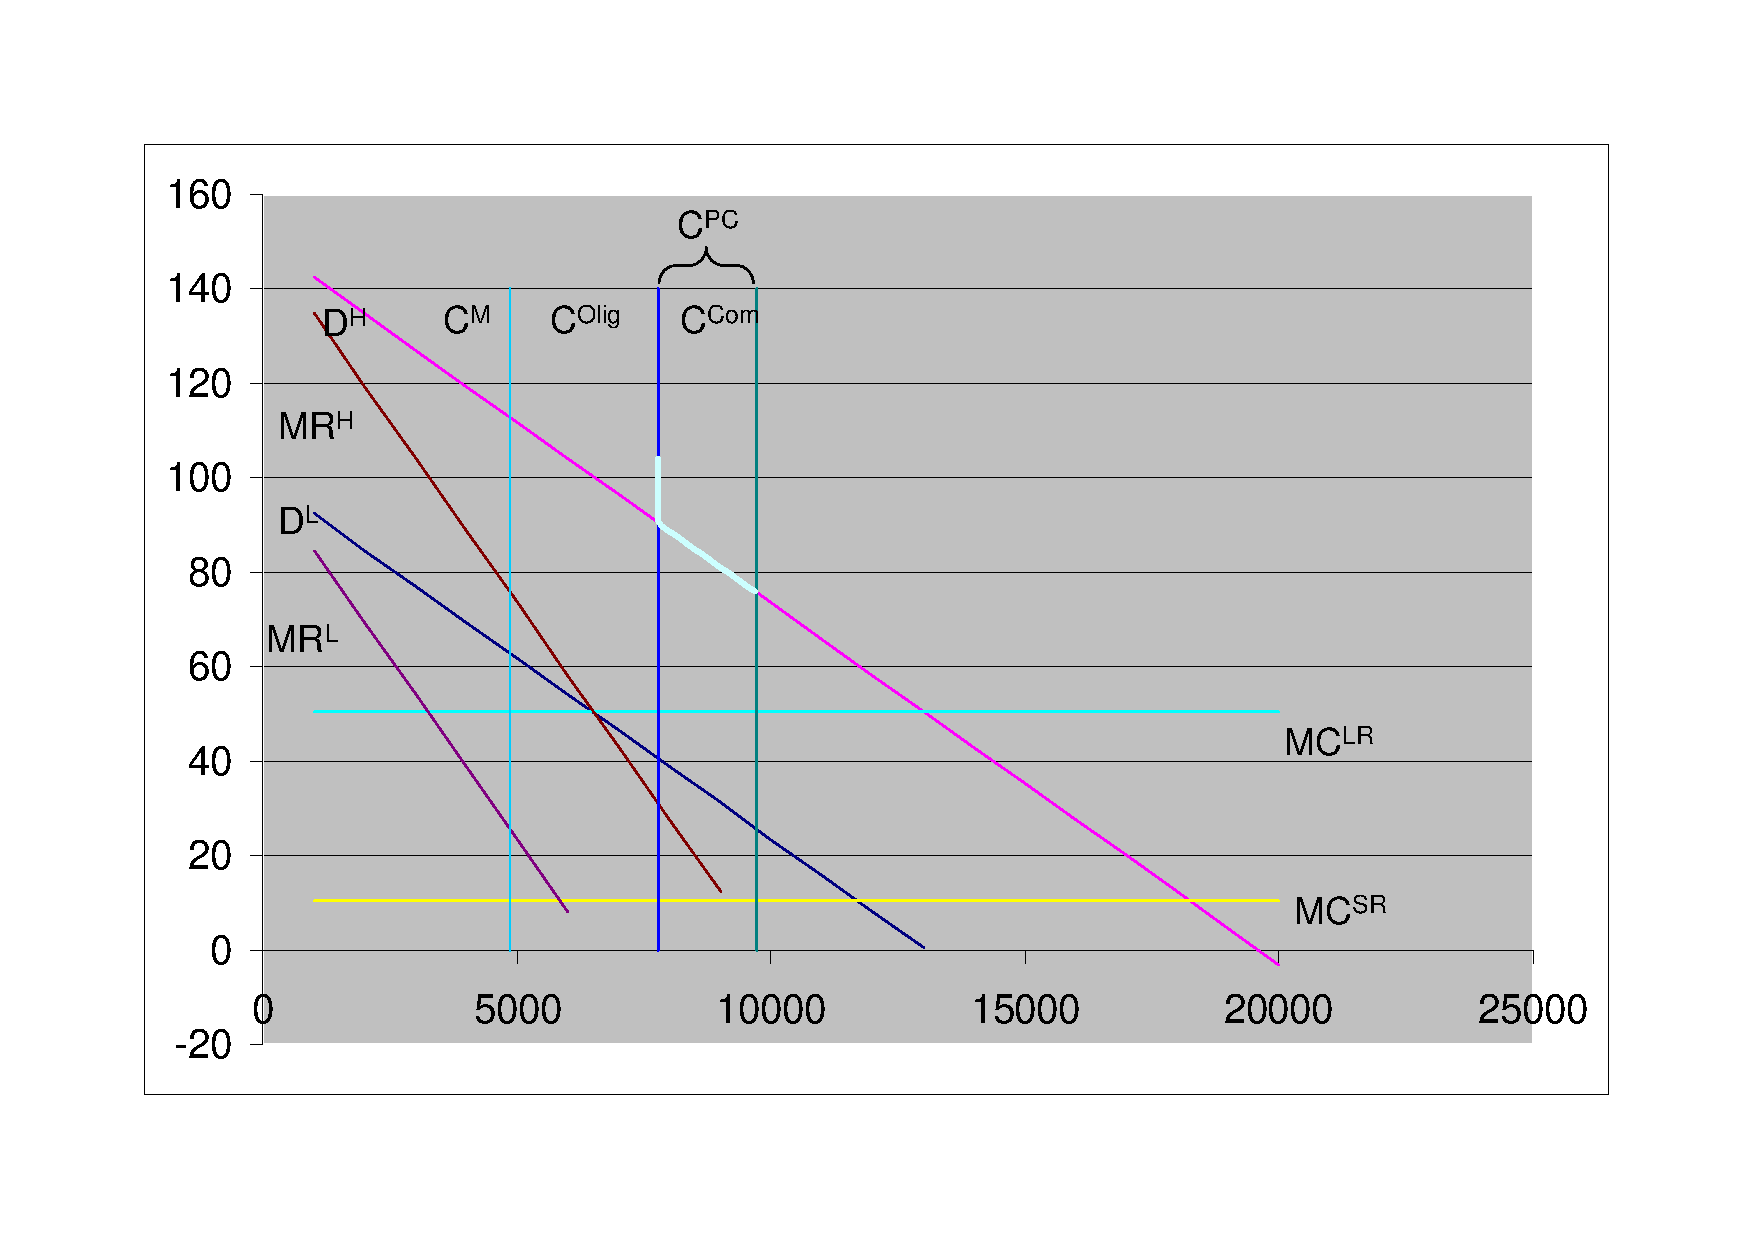
\includegraphics[width=3.0in]{capacity/eigenes_modell}
      \label{eigenes_modell}  
\\          
\scriptsize Source: own calculations
\end{figure}

So under perfect competition, one could rely on the market to provide optimal incentives for capacity investments. However, this does not mean that prices should always be equal to marginal costs, as during peak periods firms must be allowed to cover their investment costs by scarcity rents.

\subsection{Welfare, Options and Capacity Markets}

Following the intuition that scarcity rents are needed to cover investment costs, it is often argued that price caps to mitigate market power destroy investment incentives. The scarcity rents capped by the price cap are generally called the "`missing money"' in the respective stream of Literature over which \cite{Cramton2006} gives an excellent overview.
The same stream of literature argues in favor of capacity markets which should create additional investment incentives. These additional incentives should overcome the missing money problem and seem to be aimed to account for welfare considerations which are not contained into the welfare losses due to rationing which we described above. If capacity is binding, the price of electricity is equal to the willingness to pay of the marginal consumer. The consumers on the electricity wholesale market however, are not the end users but usually retailers and it might well be that they care less than their end users about electricity deliveries which had to be price rationed. A possible solution for this problem might be to make electricity retailers pay penalties for the value of lost load (VOLL). \cite{Burger2007} present a case study case study how this might be done.
An alternative setup is presented in \cite{Boom2007} where a blackout can occur in the case of which all players loose all their rents. \cite{Chao2004} show how market power is mitigated and how new investments are facilitated if option contracts are introduced. We do not account for such market features, although it might be an interesting alternative for further research.
Capacity investments have also been studied from a real option perspective which incorporates the value to delay investments by \cite{Roques2006}.

\subsection{Peak-load pricing under imperfect competition}

The seminal article when it comes to capacity choice under imperfect competition is \cite{Kreps1983} who showed that firms would choose exactly the Cournot quantities in a two stage game. \cite{Gabszewicz1997} analyze investment under demand uncertainty with quantity competition in the second stage and compare that to a Cournot game played in expected demand which they call the Cournot certainty equivalent game. These models are examples of two stage closed loop games. \cite{Grimm2007} uses an analytical closed loop model to analyze the effect of Cournot competition in the first, and Bertrand competition in the second stage for example.
How optimal incentives to invest in electricity generation equipment are distorted by an oligopolistic situation is discussed from a very practical point of view in \cite{Brunekreeft2005} for example. The discussion in \cite{Murphy2005} has been mentioned beforehand already. \cite{Genc2007}, \cite{Genc2007a} and \cite{Lise2008} discuss numerical models of electricity markets based on open loop games but do not focus on economic explanations of the effects found. As we use an open loop information structure, in our model, there is always the same mode of competition in the first and the second stage of the game which might be intuitive, as - at least in the electricity market - there is no obvious reason why firms should first interact on the basis of Cournot and then follow a Bertrand logic or vice versa.
Under imperfect competition, firms might have an incentive to reduce investments, thereby driving up the price in peak periods and increasing their profits. Of course, this only works if there are barriers to entry beyond the unit costs of investment. The effect of lower than optimal investments is depicted in Figure \ref{peak_load_insufficient}.

\begin{figure}[h]
\centering
\caption{Insufficient supply}
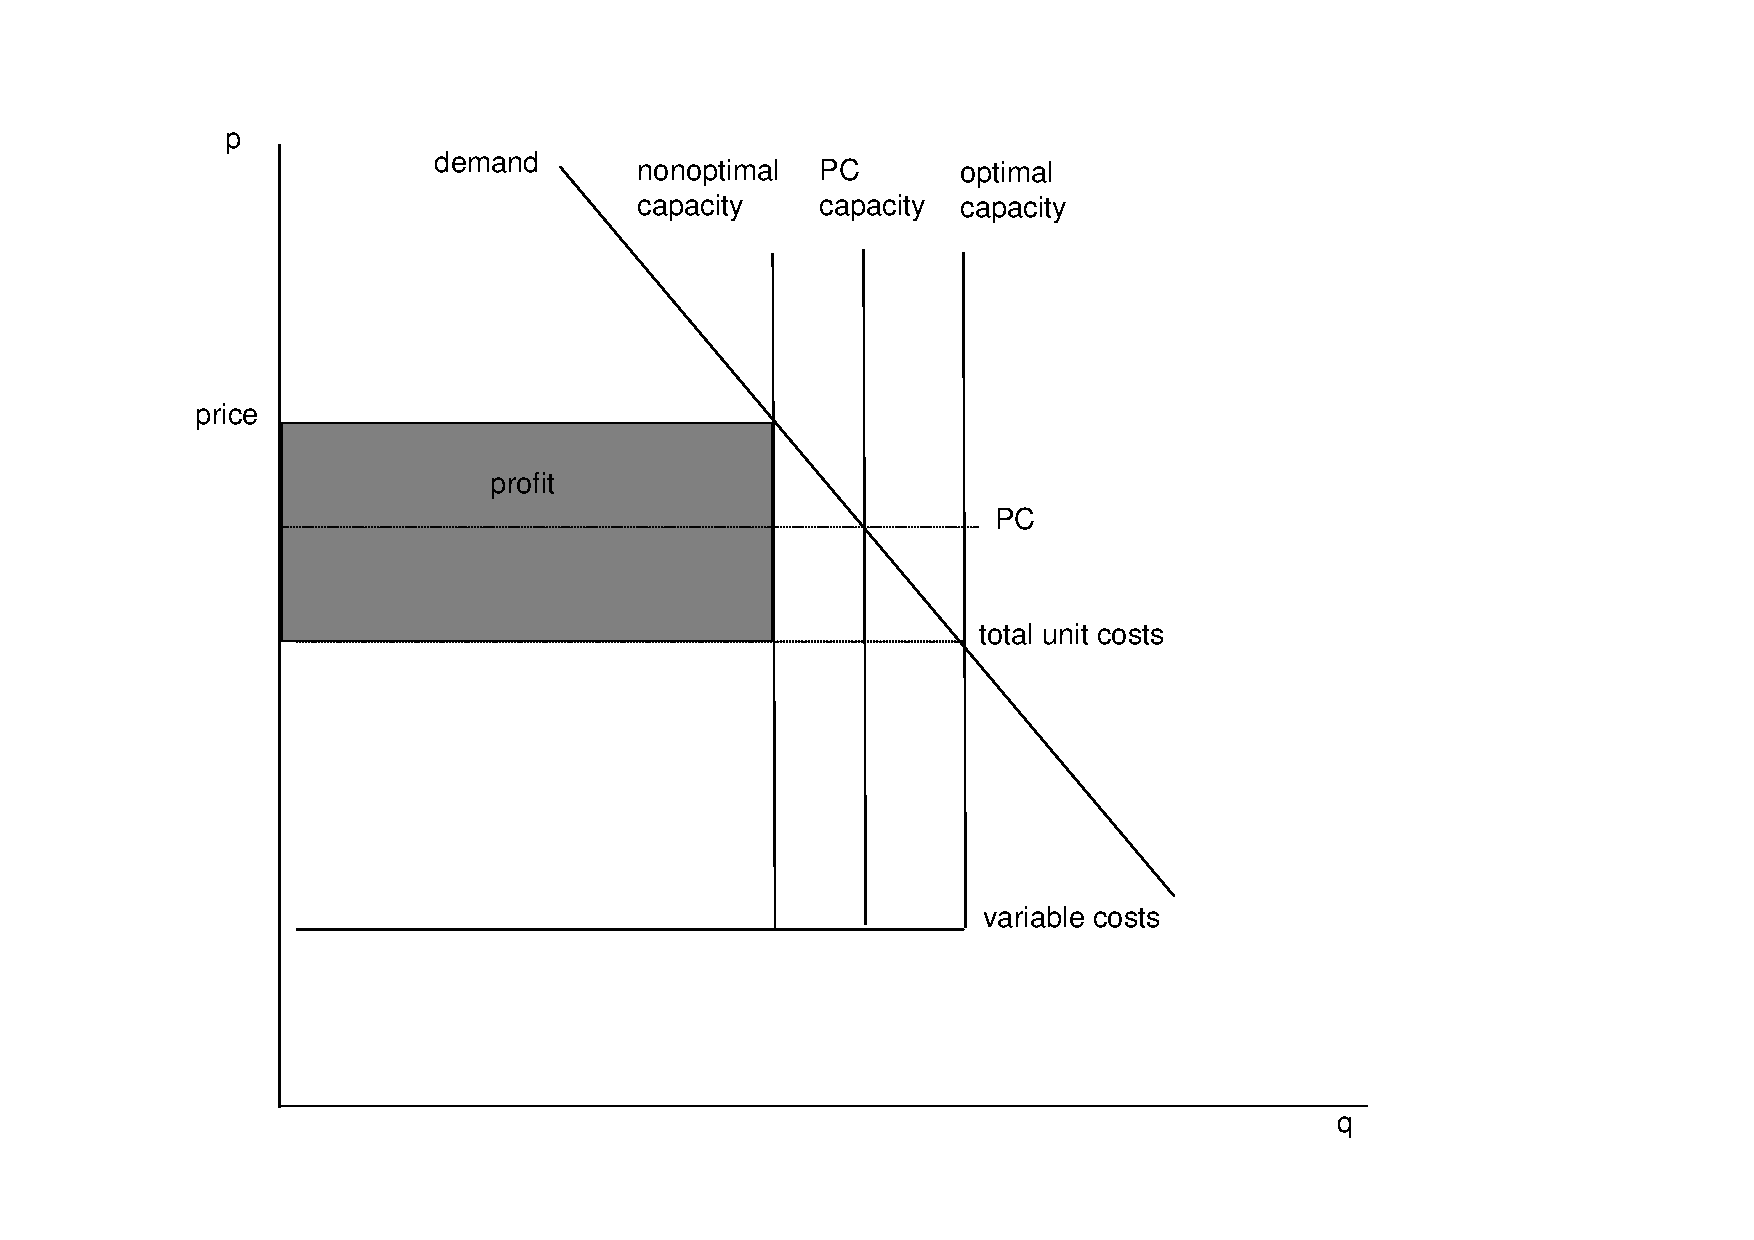
\includegraphics[width=4.2in]{capacity/insufficient_supply.pdf}
      \label{peak_load_insufficient}  
\\          
\scriptsize Source: own calculations
\end{figure}


 
Figure \ref{eigenes_modell} shows results from a simplified version of our model for the Monopoly, Oligopoly (4 Players) and the perfect competition case. It can be seen easily, that there is an underinvestment problem in the case of an oligopoly, which is somewhere between the two benchmark cases. 

%As a monopolist bases it�s decisions on his expected marginal revenue $(MR^H, MR^L)$ Je nachdem wie MR ausssieht erreicht man schneller die - steht am Zettel.

We will now use the example from \cite{Fehr1995} to illustrate the two competing effects.
While the socially optimal incentive to invest is still the same as above, a firm in an oligopolistic situation gets the following expected revenue per unit of investment:

\begin{equation*}
	\frac{1}{2} (1-\pi) (p^{op}-v) + \pi \left(w^p(K)+\frac{\partial w^p(K^*)}{\partial q}-v\right) - c
\end{equation*}

The first part of the equation stands for possible gains of the investment that might occur during low peak periods. For simplicity we assume that there is a duopoly and a probability of $1/2$ for a new unit of capacity to be utilized. This is then multiplied by the probability to not have a peak period $(1-\pi)$ and the oligopoly price minus variable costs $(p^{op}-v)$. In such periods it is possible to steal business, you would normally not have, from another firm. Such an effect can create an additional incentive to invest in capacity. In the case of multiple technologies, a firm could also invest into cheap base load plants which replace plants with higher marginal costs. %As we shall see later on, this effect can be called a strategic effect of investments as well.

The second part of the equation stands for what the investing firm looses in peak periods due to the investment. This equation is essentially the same as the condition we derived for perfect competition. The only difference is that we now write the peak price as a function of the binding capacity $p^p(K)$ and that this price now changes with capacity (and thereby quantity) changes which are illustrated by $\frac{\partial w^p(K^*)}{\partial q}$. This term measures the reduction in the peak price which is due to the decreased scarcity of capacity. This effect has to be taken into account now, as we switched from perfect competition to oligopoly.

So if the loss firms expect due to losses in the peak load market price are bigger than the gains due to more market share in off peak periods, firms will under invest as their incentive to invest is smaller than the optimal level under perfect competition. Of course, if the effect doe to business stealing is higher, firms will overinvest. So in an oligopolistic setting, firms will in general not choose an optimal level of investments.

Figure \ref{peak_load_insufficient} illustrates the effect of a price cap (PC) on investment incentives if the market price is above total unit costs due to market power. The price cap makes it impossible for the firm to increase profits by withholding or not building capacity and thereby, contrary to the missing money argument, can as well increase investments in an oligopolistic setting.

\subsection{Capacity withholding}

What is meant by capacity withholding? In the electricity market context, this term is used to describe a situation in which available capacities are not used even if the price is higher than marginal costs. In a Cournot Situation, capacity withholding naturally occurs in the short run if starting capacities are above the Cournot quantities. Such a situation can be seen in Figure \ref{cournot}. The normal Cournot equilibrium does not satisfy capacity constraints and so a constrained solution evolves from the static game.

\begin{figure}[h]
\centering
\caption{Insufficient supply}
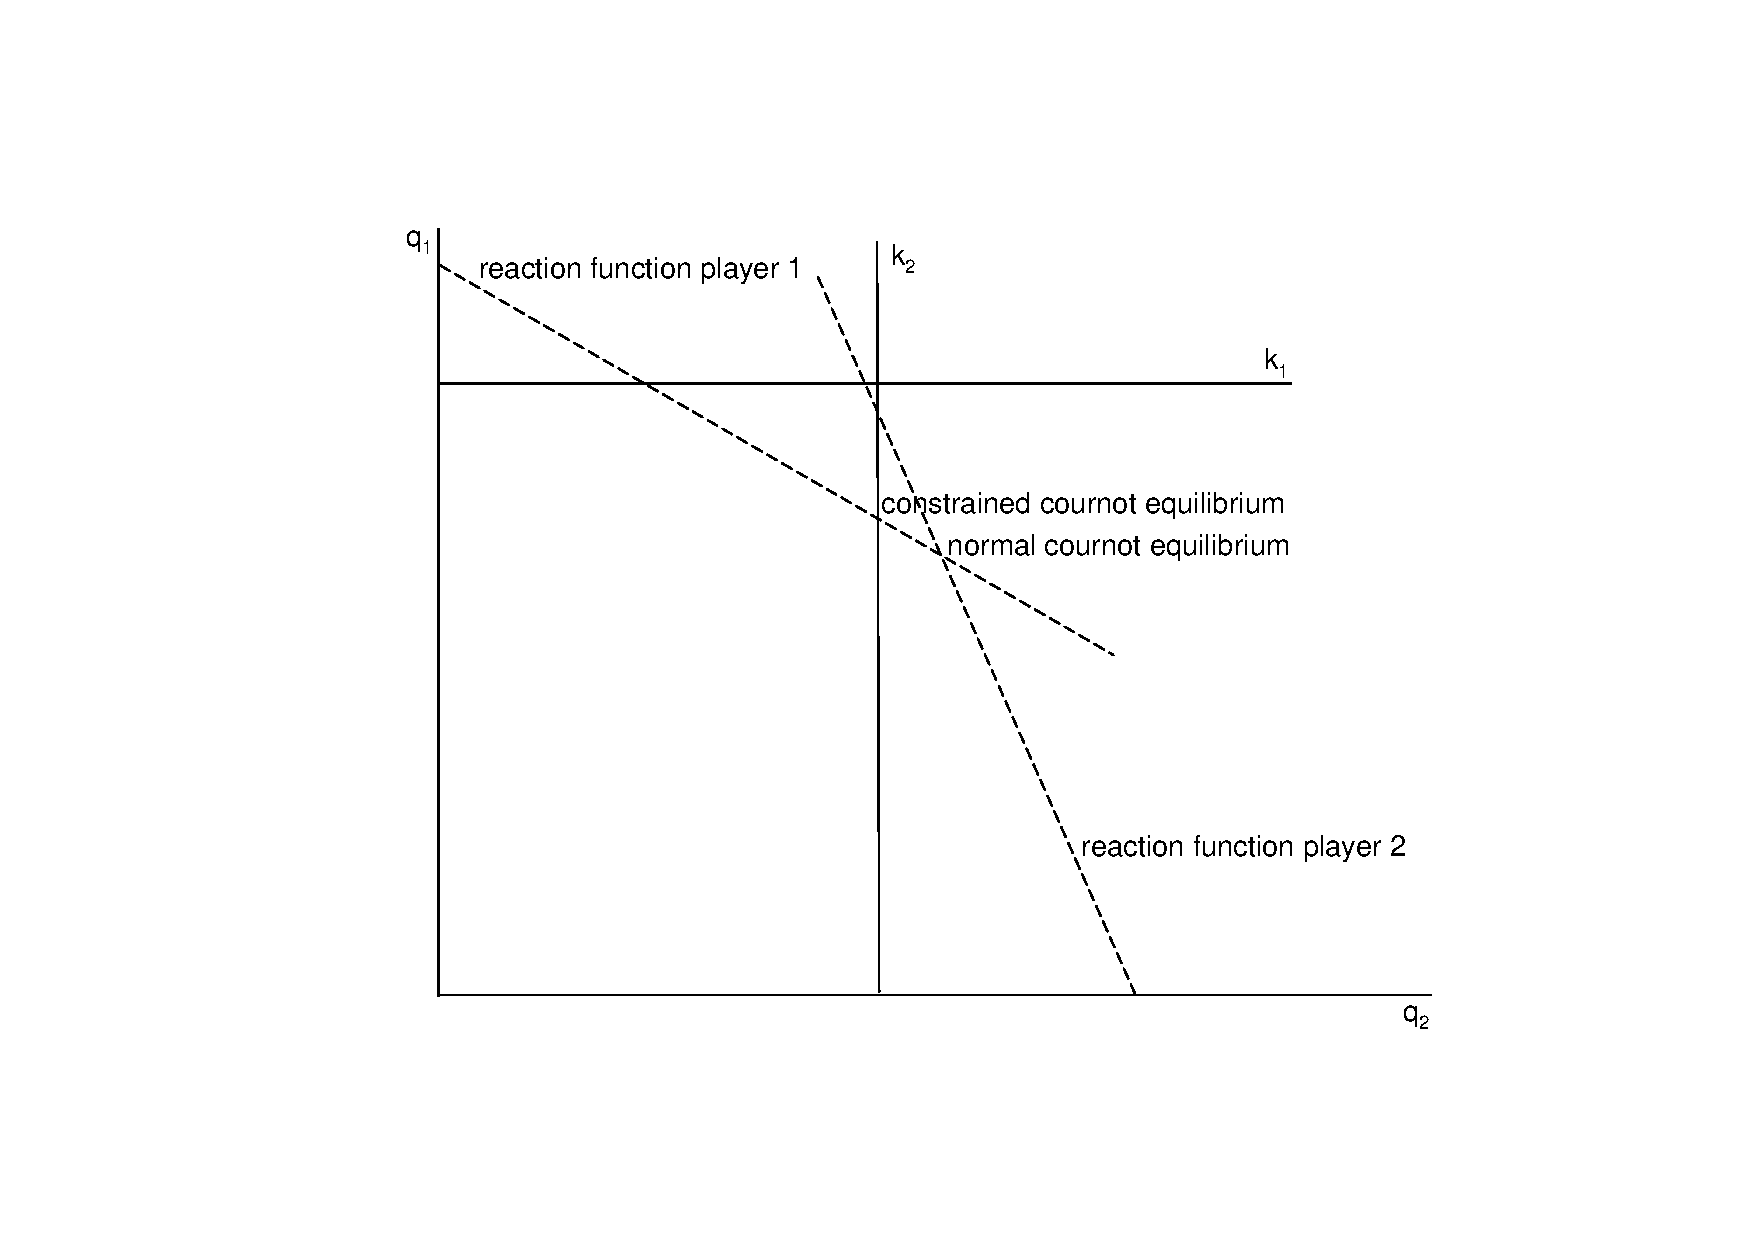
\includegraphics[width=4.2in]{capacity/Cournot.pdf}
      \label{cournot}  
\\          
\scriptsize Source: own calculations
\end{figure}

In a dynamic (open loop??????) setting however, firm one would let his capacity depreciate and firm two would invest until both capacities reach the normal cournot equilibrium. Then, there are no unused capacities any more but capacities itself are not optimal as they resemble an equilibrium with market power. 
If there is uncertainty about future demand there will always by situations with spare capacities. We illustrate this, by considering two different reaction functions, one for high and one for low demand for both players (\ref{cournot_uncertainty}). In such a case, spare capacities in peak periods become unavoidable. Please note that, in this context, uncertainty could resemble different possible loads coming from a load duration curve, or uncertainty about demand growth.

\begin{figure}[h]
\centering
\caption{Insufficient supply}
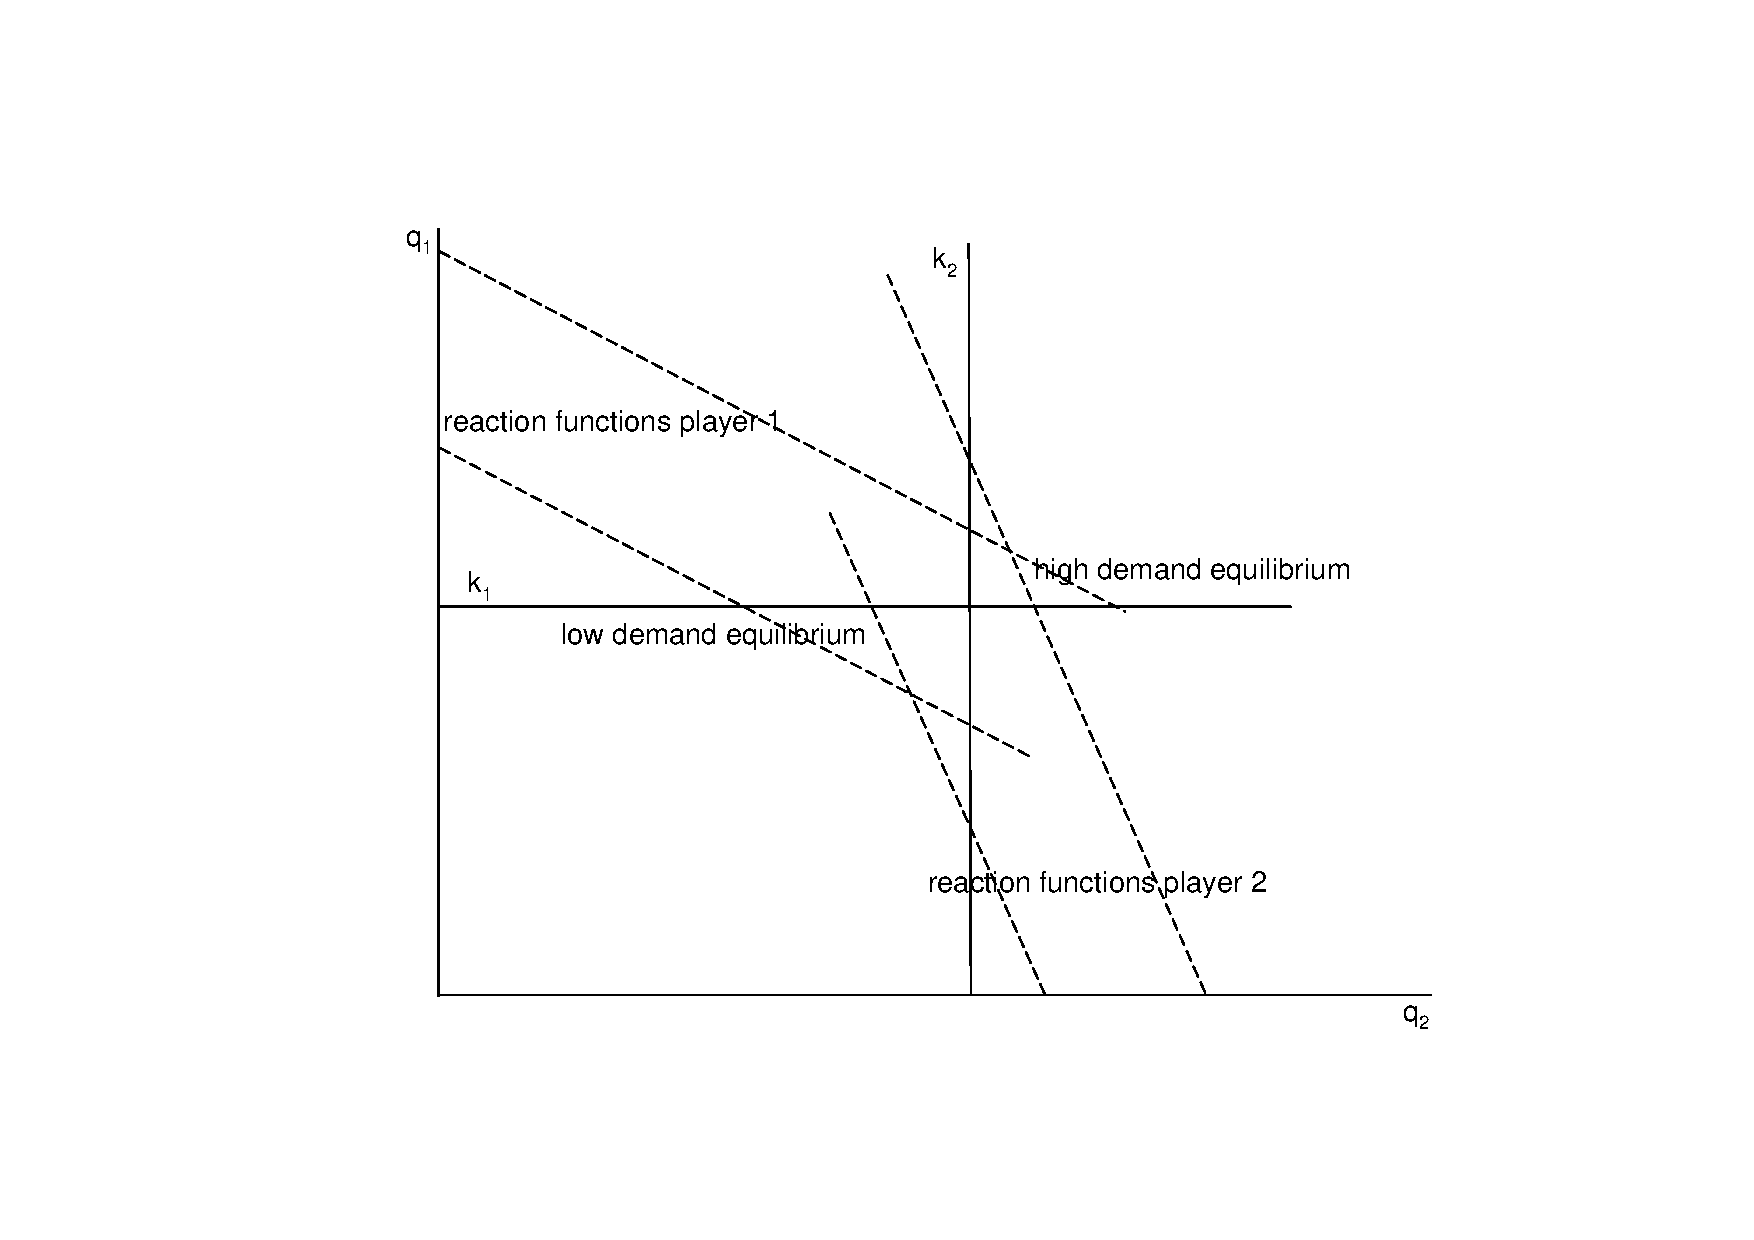
\includegraphics[width=4.2in]{capacity/cournot_uncertainty.pdf}
      \label{cournot_uncertainty}  
\\          
\scriptsize Source: own calculations
\end{figure}

%If there is market power, the above mentioned optimality result does not necessarily hold as prices above marginal costs may induce overinvestments. The situation of too high prices is depicted in Figure \ref{peak_load_toohigh}.

%\begin{figure}[h]
%\centering
%\caption{Imperfectly competitive spot pricing}
%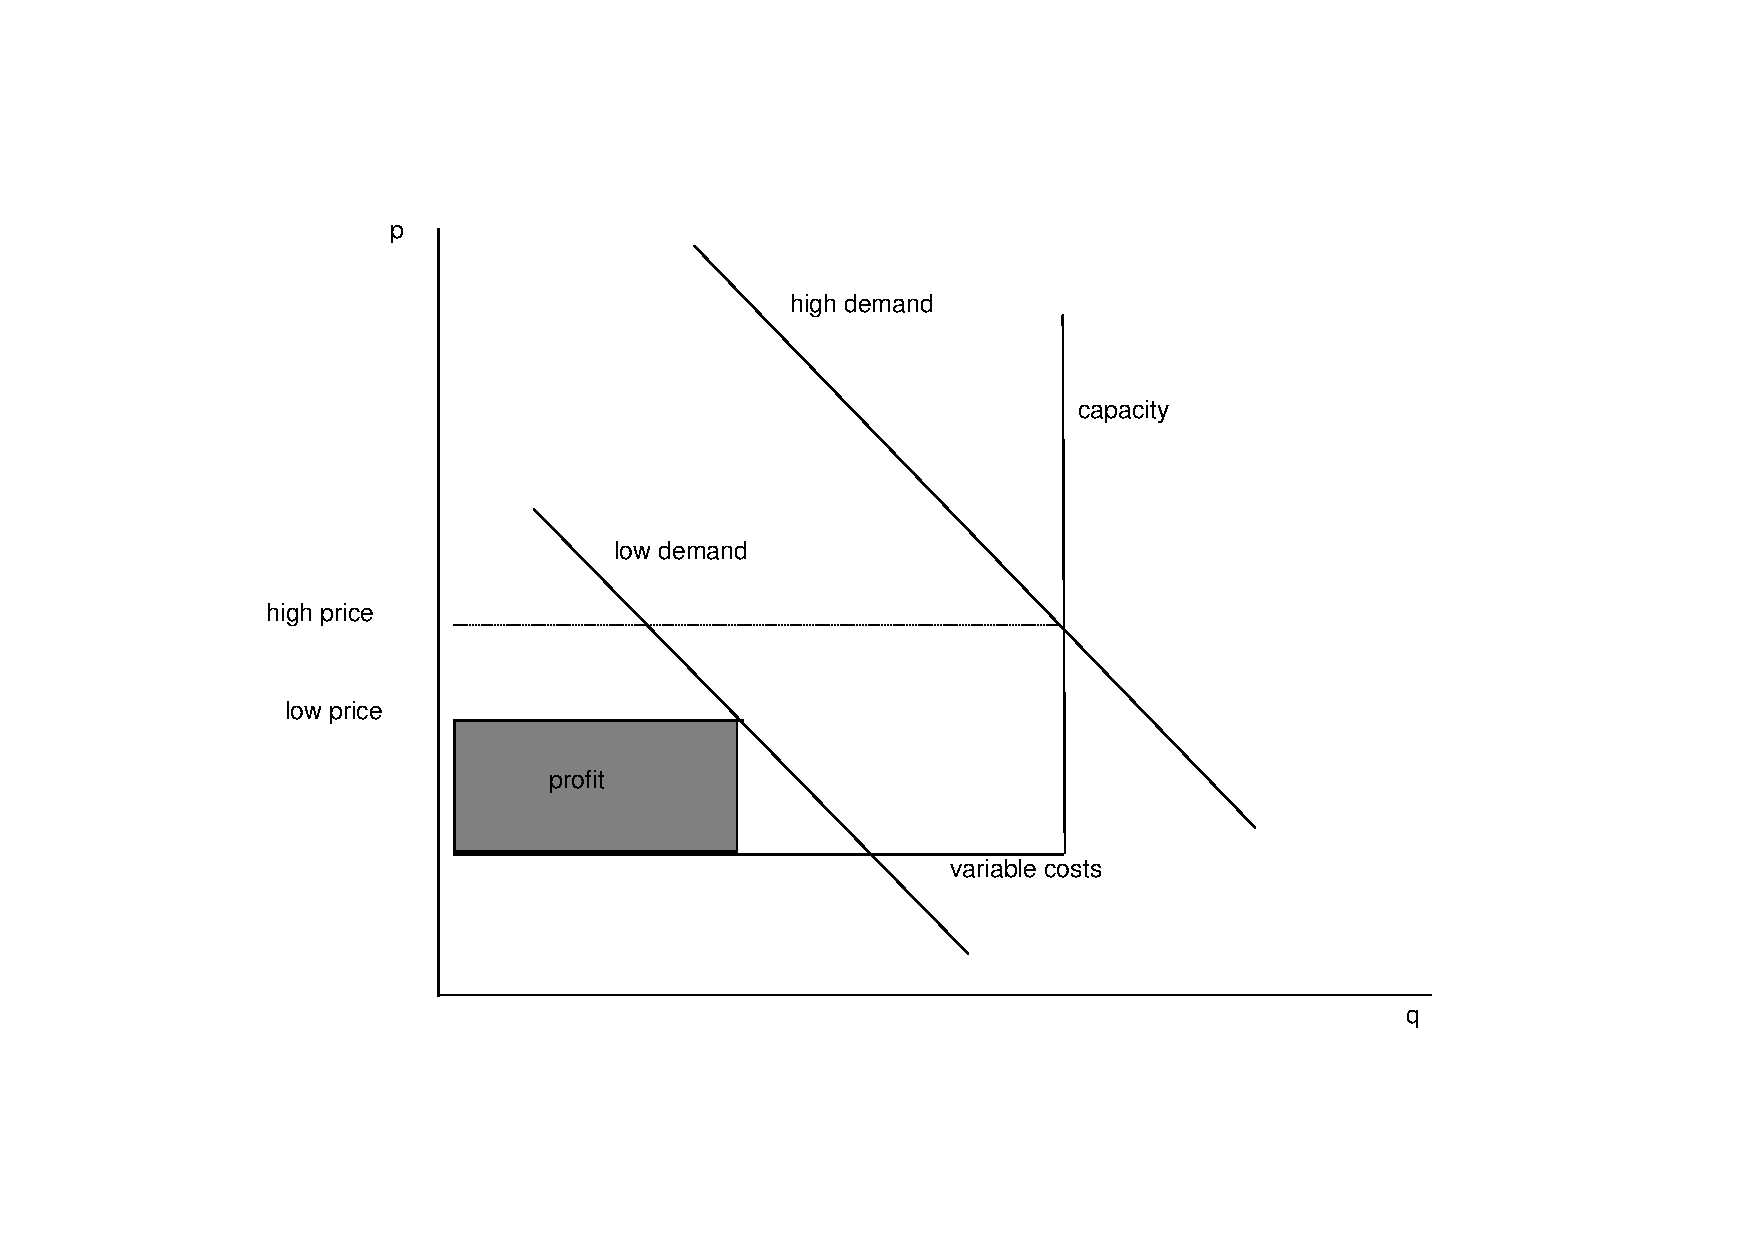
\includegraphics[width=3.0in]{capacity/imperfect_spot_pricing.pdf}
%      \label{peak_load_toohigh}  
%\\          
%\scriptsize Source: \cite{Fehr1995}
%\end{figure}

%The premium of the market price in peak periods ($p^p$) over marginal costs in peak periods, multiplied with the chance of actually having a period of high demand, reflects the value of increasing capacity by one unit.  The value of increasing capacity by one unit must equal capacity costs per unit. If the condition
%$$(p^p-v)\times\pi=c$$
%is met, social surplus is maximized and costs are minimized. A profit maximizing firm under perfect competition would invest until exactly this condition is satisfied. 

%To be able to assess the strength of the different effects, we set up a realistic numerical model in the next section. %As we shall see later on, in a two stage game, strategic effects can be accounted for in different ways which has an effect on the predictions made.

%\subsection{Optimal Technology Mix}

%If demand were certain and constant, only one technology (the one which reaches the lowest possible costs in a standard cost minimization problem with capacity costs and operating costs as inputs) would be used \citep[see][pg. 183]{Chao1983}. This can be seen in the following graph (\ref{technology_choice_chow}) in which a standard cost minimization problem with capacity costs and operating costs as inputs and different technologies are shown. The minimal cost combination given input prices would be technology one. But when demand is uncertain or variable and the output is nonstorable some idle capacity becomes inevitable. This makes less capital intensive technologies such as 2 and 3 more attractive which would be dominated without fluctuations. However, all technologies which are not on the lower envelope are still inferior.

%\begin{figure}[h]
%\centering
%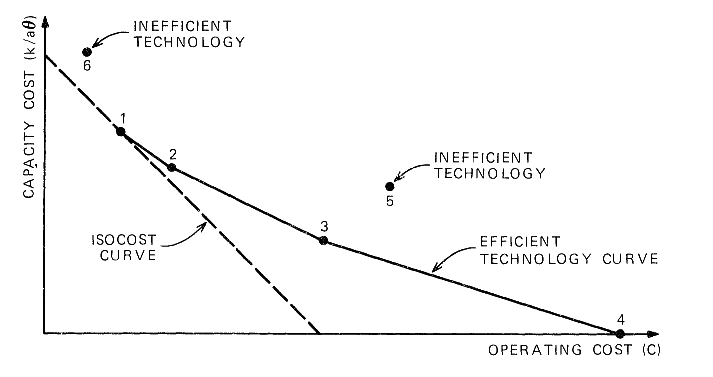
\includegraphics[width=.5\textwidth]{capacity/technology_choice_chow}
%      \label{technology_choice_chow}            
%      \caption{different technologies}
%       source: Chow (1983)
%\end{figure}

%\cite{sherali1982} present a graphical illustration on how to find the optimal mix of different technologies if demand varies. Figure \ref{technology_choice_sherali} \textbf{b} shows the so - called load duration curve which plots the hours of the year ordered according to their energy demand. It can be seen, that only during a few hours of the year demand is very high. Figure \ref{technology_choice_sherali} \textbf{a} shows the cost curves of three different technologies. Technology three has low yearly fixed costs ($c_3$) and high variable costs ($f_3$) so if it would be used for more than $\alpha_{23}$ hours in a year it would be cheaper to use technology two instead. For most of the time of the year, it is actually cheaper to use technology one only which has fairly high fixed but low variable costs. The condition of when one technology becomes cheaper than the other is the same than the one derived by \cite{chow1983} (who also adds an additional stochastic element however). This condition for an optimal technology mix has first been advanced by \cite{Turvey1968}. Also \cite{Pineau2007} uses this condition.

%\begin{eqnarray}
%	c_1 + f_1 \alpha_{12} = c_2 + f_2 \alpha_{12}
%	\alpha_{12} = \frac{c_2-c_1}{f_1-f_2}
%\end{eqnarray}

%This so called optimal running time can be translated into optimal investments into capacity of technology one two and three as can be seen in figure \ref{technology_choice_sherali} \textbf{b}.

%\begin{figure}[h]
%\centering
%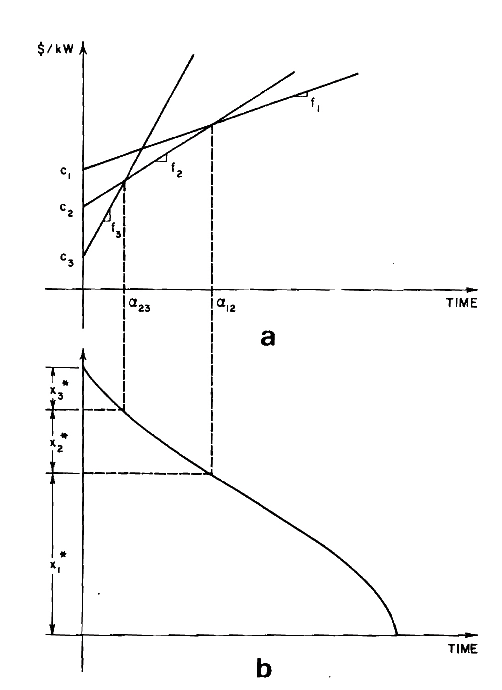
\includegraphics[width=.5\textwidth]{capacity/technology_choice_sherali}
%      \label{technology_choice_sherali}            
%      \caption{the load duration curve and cost curves - graphical determination of the optimal technology mix}
%      source: Sherali et. al. (1982)
%\end{figure}

%What can be seen here is that which kind of capacity is optimal to be built depends on where demand actually increases. It is an unresolved issue whether competition and markets, be it perfect competition or imperfect forms alter the technology mix firms have an incentive to install in any way.



%%% Local Variables: 
%%% mode: latex
%%% TeX-master: "../eem08"
%%% End: 

\section{Strategic capacity investment decisions under imperfect competition}

\subsection{Cournot solution}

\subsection{Dynamic games and information structures}


\clearpage
\section{Conclusion}
\label{sec:conclusion}

We have presented a stochastic dynamic equilibrium model for the German electricity market. The multi-stage stochastic optimization problem was formulated with the so-called compact notation. The scenario generation was based on realistic price and load data. The major contribution of this paper is the better approximation of the load duration curve, a more compact notation and the practical application example for the German electricity market.

Further research could include the time evolution of costs and more detailed forecasts for the development of the electricity load.

%%% Local Variables: 
%%% mode: latex
%%% TeX-master: "gencapinvest"
%%% End: 


%\AtBeginSubsection[]
%{
%  \begin{frame}<beamer>
%    \frametitle{Outline}
%    \tableofcontents[current,currentsubsection]
%  \end{frame}
%}





\section{References}
\scriptsize

\begin{frame}[allowframebreaks]
      \frametitle<presentation>{References}

      \begin{thebibliography}{8}

\beamertemplatebookbibitems
\bibitem{Haurie2005}
Alain Haurie and Georges Zaccour
\newblock Dynamic Games: Theory and Applications
\newblock {\em Springer}, 2005

%\framebreak

\beamertemplatearticlebibitems

\bibitem{Chaton2003}
Corinne Chaton and Joseph A. Doucet
\newblock Uncertainty and Investment in Electricity Generation with an Application to the Case of Hydro-Quebec 
\newblock{\em Annals of Operations Research}, 120(1):59-80, 2003
    
\bibitem{Genc2007}
Talat S. Genc and Stanley S. Reynolds and Suvrajeet Sen
\newblock Dynamic oligopolistic games under uncertainty: A stochastic programming approach
\newblock {\em Journal of Economic Dynamics and Control}, 31(1):55-80, 2007 

\bibitem{Murphy2005}
Frederic H. Murphy and Yves Smeers
\newblock Generation Capacity Expansion in Imperfectly Competitive Restructured Electricity Markets
\newblock {\em Operations Research}, 53(4):646--661, 2005
	
\bibitem{Pineau2003}
Pierre-Olivier Pineau and Pauli Murto
\newblock An Oligopolistic Investment Model of the Finnish Electricity Market
\newblock{\em Annals of Operations Research}, 121(1):123-148, 2003

\bibitem{Pineau2007}
Pierre-Olivier Pineau and Georges Zaccour
\newblock An Oligopolistic Electricity Model with Interdependent Market Segments
\newblock{\em The Energy Journal}, 28(3):, 2007

\bibitem{Salant1982}
Stephen W. Salant
\newblock Imperfect Competition in the International Energy Market: A Computerized Nash-Cournot Model \newblock{\em Operations Research}, 30(2): 252-280, 1982

\bibitem{Ventosa2005}
Mariano Ventosa, Alvaro Baillo, Andres Ramos and Michel Rivier
\newblock Electricity market modeling trends
\newblock{\em Energy Policy}, 33(7): 897-913, 2005

   \end{thebibliography}
\end{frame}

\end{document}